\documentclass{article}
\usepackage{tikz}
\usepackage[left=0.5cm,right=0.5cm]{geometry}

\pagestyle{empty}
\begin{document}
\thispagestyle{empty}
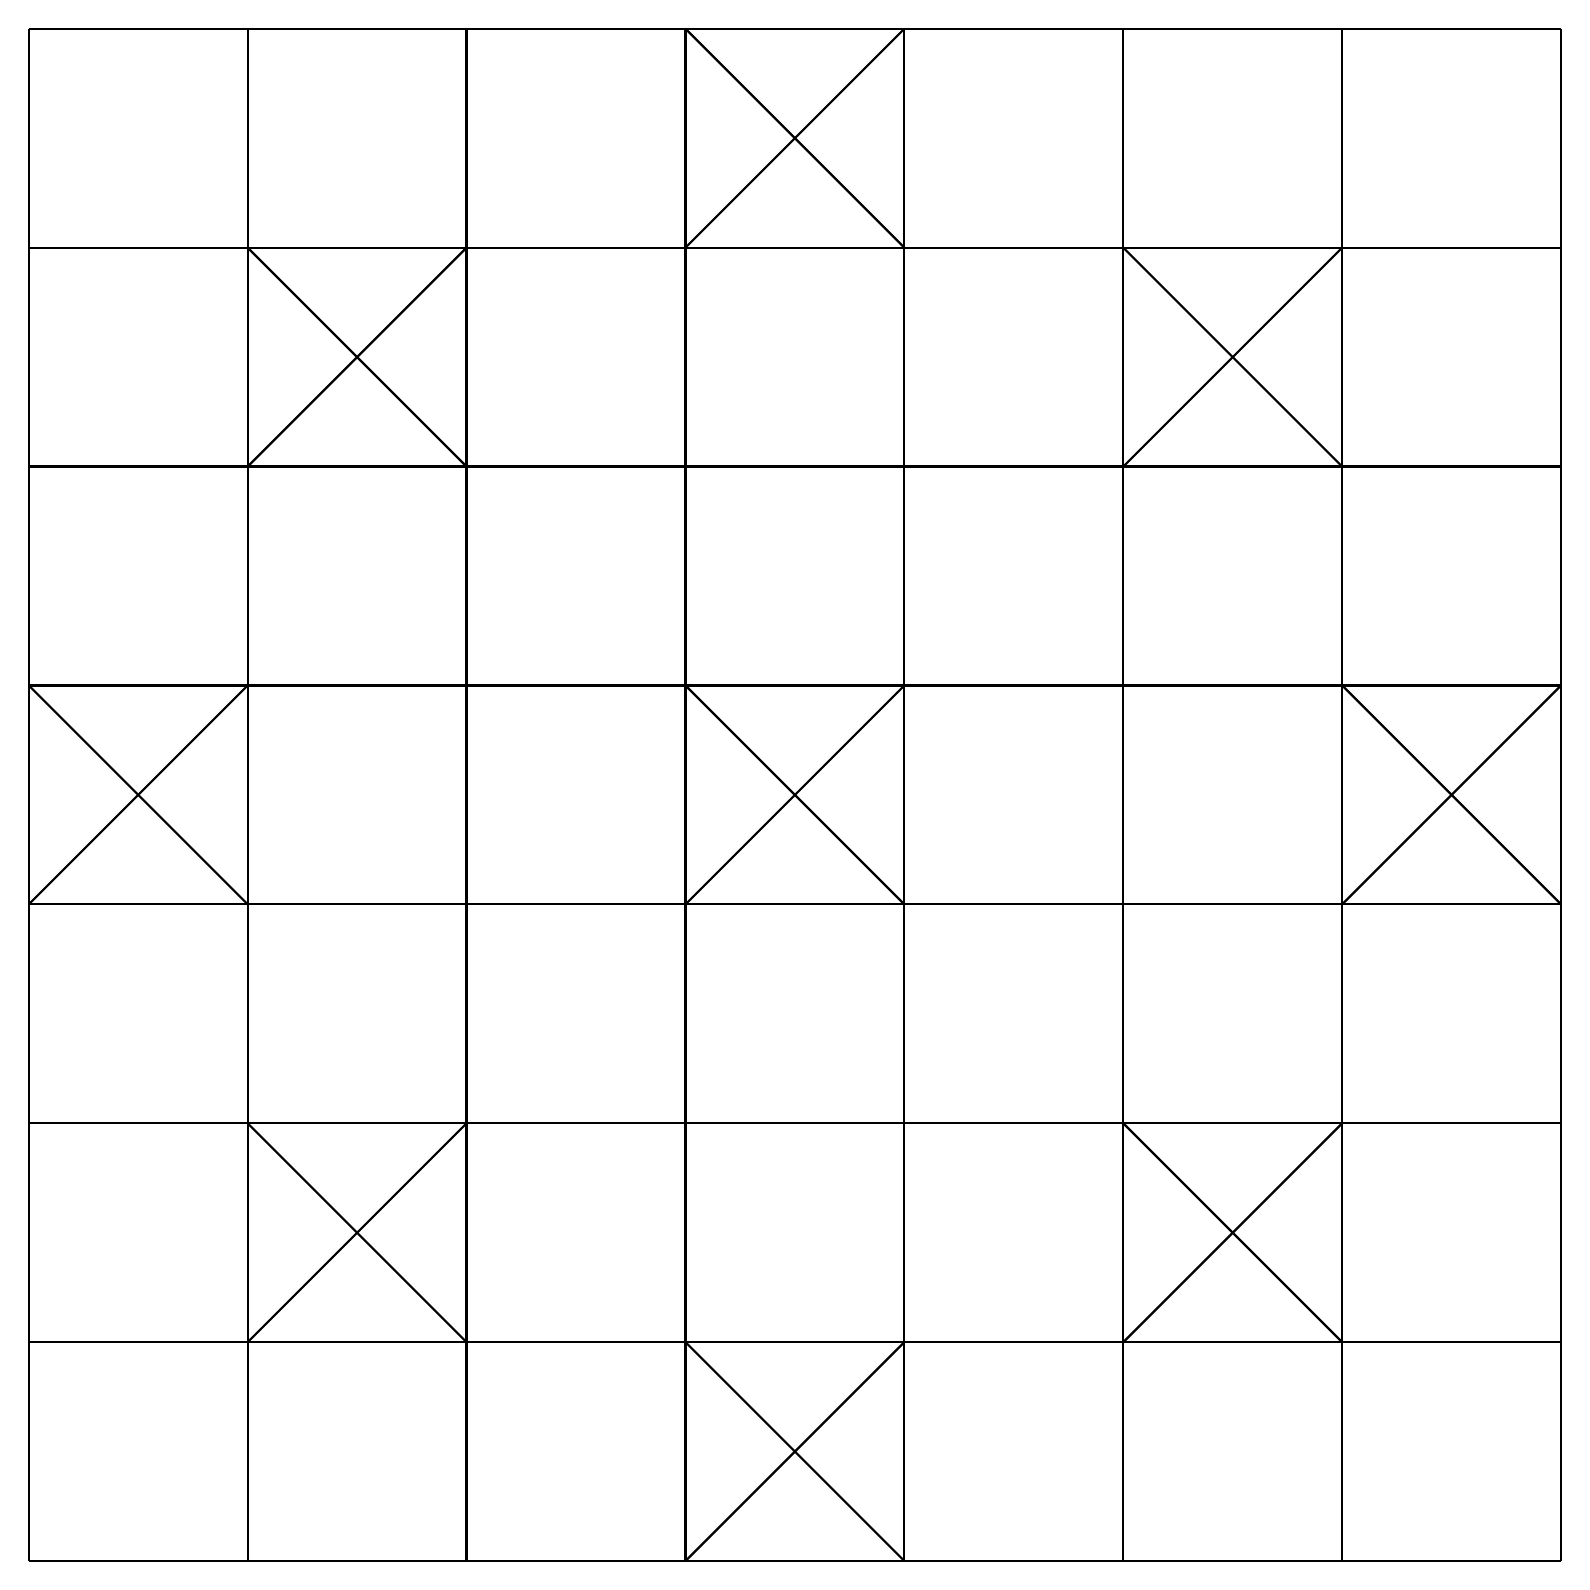
\begin{tikzpicture}[thick, scale=2.78, every node/.style={scale=2.78}]

%follow this pattern
%  \draw (a, b) - (c, d)
%  \draw (c, b) - (a, d)

%follow this pattern (with calculations)
    %  \draw (x, y+1) - (x+1, y)
    %  \draw (x+1, y+1) - (x, y)


%safe place means malai_ta
\newcommand{\safeplacemarker}[2]{
        \draw (#1,#2+1) -- (#1+1, #2);
        \draw (#1+1,#2+1) -- (#1, #2);
}
\draw (0,0) grid (7,7);

%%center
\safeplacemarker{3}{3}

%%next round
\safeplacemarker{1}{1}
\safeplacemarker{1}{5}
\safeplacemarker{5}{1}
\safeplacemarker{5}{5}

%%outermost round
\safeplacemarker{0}{3}
\safeplacemarker{3}{0}
\safeplacemarker{3}{6}
\safeplacemarker{6}{3}


\end{tikzpicture}
\end{document}
